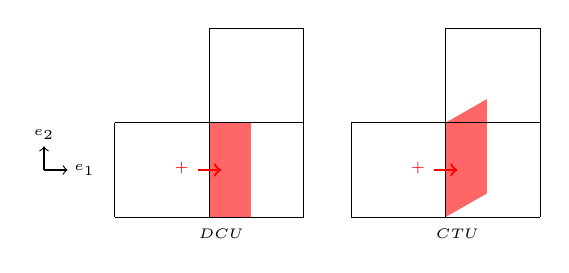
\begin{tikzpicture}[scale=0.6]
  \fill[Red!60] (0,0) rectangle (.875,-2);
  \draw (-2,0) -- (2,0.);\draw (0.,2) -- (0,-2.);\draw (0,2) -- (2,2);
  \draw (-2.,-2.) -- (2.,-2.);\draw (2,2.) -- (2,-2.);\draw (-2,-2) -- (-2,0);
  \begin{tiny}
    \draw[->,thick,Red] (-.25,-1.) node [left] {$\Ac^+$} -- (.25,-1.) ;
    \draw[->] (-3.5,-1.) -- (-3,-1.) node[right] {$\vect{e}_1$};
    \draw[->] (-3.5,-1.) -- (-3.5,-0.5) node[above] {$\vect{e}_2$};
    \node at (0.25,-2.35) {$DCU$};
  \end{tiny}
  \begin{scope}[shift={(5.,0.)}]
    \fill[Red!60] (0,0) rectangle (.875,-2);
    \fill[Red!60] (0,0) -- (.875,0) -- (.875,.5) -- (0.,0.); %% Red triangle
    \fill[white] (0,0-2) -- (.875,0-2) -- (.875,.5-2) -- (0.,0.-2); %% White triangle
    \draw (-2,0) -- (2,0.);\draw (0.,2) -- (0,-2.);\draw (0,2) -- (2,2);
    \draw (-2.,-2.) -- (2.,-2.);\draw (2,2.) -- (2,-2.);\draw (-2,-2) -- (-2,0);
    \begin{tiny}
      \draw[->,thick,Red] (-.25,-1.) node [left] {$\Ac^+$} -- (.25,-1.) ;
      \node at (0.25,-2.35) {$CTU$};
    \end{tiny}    
  \end{scope}
\end{tikzpicture}

%%% Local Variables:
%%% mode: latex
%%% TeX-master: "../../presentation"
%%% End:
